%!TEX root = cscw2019-comic.tex

% what is the problem?

% why is it important? what is the impact? what motivates?

% who else has done it?
% what did you do?

\section{introduction}
\label{sec:introduction}

\begin{wrapfigure}{R}{0.23\textwidth}
    \centering
    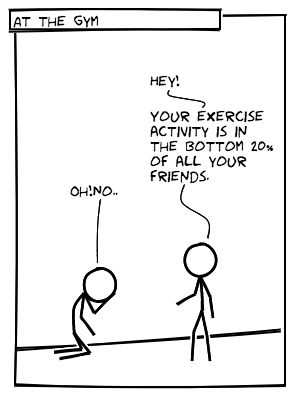
\includegraphics[width=0.21\textwidth]{figures/intro_new.png}
  \vspace{-10pt}
  \caption{The figure highlights information framing and the use of an abstract comic form.} \label{fig:intro}
  \vspace{-10pt}
\end{wrapfigure}

From online charitable donation to open source software development, technology advancement expands people's ways to contribute to public goods. Research have shown that such collective action is essential to social prosperity ~\textcite{}. However, since public goods cannot be confined solely to those who have paid for it, there is no tangible utility for people to contribute ~\textcite{}. Without individual's contribution, some public goods such as knowledge and charity may scare. Therefore, extensive efforts had been put to understand how to nudge individuals to join collective actions.

Although people can take "free-ride" on public goods, intrinsic motives such as altruism ~\textcite{}, reciprocity~\textcite{}, and personal satisfaction ~\textcite{} drive people to contribute to public goods. On the other hand, when people making decision on devoting their money, time, and efforts to public goods, there were factors from outside world influencing other than pure good faith. Nudges from the organizations or governments are one of the most influential factors. Those nudges were often in a pure-textual form and framed to persuade people for a specific causes. Although such persuasive messages look very simple, their persuasive power should not be underestimated.
For example, Wikipedia, world's largest free encyclopedia that written by volunteers, raised over 30 million funds in 2017 through a text banner on the top of each article. 

To further equip mesages with adequate persuasive power, persuasion reserachers found human often take heuristics when making decisions and those heuristics can be exploited by adversaries as the bait to lure an individual into a behavior that counter to his/her best interests. Cialdini called those baits as psychological principles of influence. Studies concluded seven principles including, authority, commitment, liking, perceptual contrast, reciprocation, scarcity, and social proof. With such influence weapens, persuader can easily frame the original messages in a different ways that can be perceived as more convcing. For example, in a well known experiment on the design of signs for towel reuse,~\textcite{goldstein2008room} showed that use of social proof in the message had a significant impact on towel re-use, when compared to the standard sign that asks us to re-use towels to save water. 

While those persuasive techniques have made persuasive messages appeal more, human beings show significant resistance to coorprate in collective actions and contribute to public goods. Although there may be confounds that explain away poor adoption, including, message timing~\textcite{Fogg2009} (i.e. when we deliver the message), time scarcity~\textcite{Janssen2016} (i.e. we don't have time to digest the information), viewing messages on smartphones~\textcite{Kim2016} (screen is too small to communicate effective visualizations), rethinking the textual form of the message for easier consumption in the context of behavior change has been largely unexplored.

In this study, we explored a novel way to synthesis persuasive messages, ''abstract comic'' \footnote{We use ``comic form'' as opposed to the more formal ``graphic form'' to avoid any confusion with other visual representations of data, including charts and diagrams.}. We compared the persuasive power of the same message (e.g. "Would you like to donate to support the Organization for Autism Research?") in two different forms, pure-textual and abstract comic, that aim to encourage individual to contribute to the public goods (e.g. making online charatible donation decisions). 
 
Two ideas underpin this paper: the comic form and information framing. First, comics is a sophisticated form of art~\textcite{scott1993understanding} that popular across cultures allowing for use of humor and affect in communication. Effectively communicating emotion and affect is key to nudge people to contribute to the public goods since the main drives for pro-social behaviors or decisions were also intrinsic, e.g. altruism. Moreover, we focus on abstract comic representations (see~\Cref{fig:intro}). By an abstract representation, we mean that the comic de-emphasizes character detail (face, eyes etc.), or details about the locale. As~\textcite{scott1993understanding} points out, using abstract representations for the comic allows the reader to project themselves onto the comic character which may make the persuadee less resistent to receive and digest the message. Equally importantly, if we wish to algorithmically synthesize comic-style messages, abstract representations allows for a straightforward synthesis and for use in a wide variety of contexts. Furthermore, comics are usually in the form of juxtaposed sequences of panels of images or a standalone single image. Beside the graphical representation, textual elements such as speech balloons, captions, and onomatopoeia often communicate dialogue, narration, sound effects, or other information. Existing work shows that comics can effectively convey meanings \textcite{McDermottPB18,cary2004going,scott1993understanding}. Therefore although embellishing a text message using a comic form appears to be a ``Supposedly Irrelevant Factor''~\textcite{Thaler2015}, that ought to make no difference to a decision maker since the comic offers no additional information, becuase 

we believe abstract comic can effective communicate 

%emphaized in encounrge pro-social behaviors 

As a consequence, we hypothsized,
\begin{description}
 \item[RQ-1]: Are statistical facts about individual behavior more persuasive when presented through abstract comic form?
 \item [RQ-2]: What is the effect of social proof in modulating comic persuasiveness?
\end{description} 


In the our study on persuasion ($n=307$), we examined if participants are persuaded to donate to a charity when presented with a three panel comic; we also performed an additional experiment that combined the idea of the social proof with the comic message.

We analyzed the results of both studies using a hierarchical Bayesian framework. Consistent with the observations by~\textcite{Kay2016}, we believe that beyond the role of Bayesian analysis on the issue of replicability, by shifting the question from the binary ``did it have an effect?'' to ``how strong is the effect?'' is important in small-$n$ studies common to HCI.


We organize the rest of this paper as follows: we first discuss related work and motivating ideas. Then, we present our sutdy design and result. Then, we discuss the implications of our results, including study limitations, followed by conclusions.


%First, work in Behavioral Economics~\cite{tversky1992advances,tversky1981framing} shows that how we frame the text matters and can cause preference reversal. Briefly, individuals show different preferences to statements with identical information due to risk aversion.
% (e.g. ``if you take the plane, there is a 50\% chance that you will fall ill'' vs. ``if you take the plane there is a 50\% chance that you will be healthy''; the former is more salient due to risk aversion). We plan to use frames to represent statistical facts.
 %Second, work in Psychology shows that individuals' decisions are guided by social norms~\cite{goldstein2008room,schultz2007constructive}.
%  In a well known experiment on the design of signs for towel reuse,~\textcite{goldstein2008room} showed that use of social norms in the message had a significant impact on towel re-use, when compared to the standard sign that asks us to re-use towels to save water. In a related study,~\textcite{schultz2007constructive} demonstrated the positive impact of comparing one's energy consumption patterns with that of one's neighbors. Today, many households in the U.S. receive bills from their utility companies comparing their energy use to their neighbors as a consequence of this study. In our paper, we use this idea of the ``social proof'', by comparing the performance of an individual to that of her friends.
 %Finally, we use comics in abstract form to communicate. Comics is a sophisticated form of art~\cite{scott1993understanding} that popular across cultures allowing for use of humor and affect in communication. We focus on abstract comic representations (see~\Cref{fig:intro}). By an abstract representation, we mean that the comic de-emphasizes character detail (face, eyes etc.), or details about the locale. As~\textcite{scott1993understanding} points out, using abstract representations for the comic allows the reader to project themselves onto the comic character.
 %Equally importantly, if we wish to algorithmically synthesize comic-style messages, abstract representations allows for a straightforward synthesis and for use in a wide variety of contexts.



%Are text messages (e.g. ``you've exercised 25\% more than you did last week'') more persuasive when expressed in comic\footnote{We use ``comic form'' as opposed to the more formal ``graphic form'' to avoid any confusion with other visual representations of data, including charts and diagrams.} form? Embellishing a text message using a comic form appears to be a ``Supposedly Irrelevant Factor''~\cite{Thaler2015}, that ought to make no difference to a decision maker since the comic offers no additional information.

%The notion of behavior change motivates us to address this question. As the quantified self movement~\cite{Epstein2014,Choe2014} illustrates, people have an enduring sense of curiosity about their lives, and develop different processes to instrument (e.g. using a wearable device) and to reflect on data gathered about their activities. Individuals use this information (``checked in at the gym twice this week''), to take decisions to change behavior (e.g. ``exercise more''; ``eat healthy'').
% In macro-scale collective action dilemmas, individual contributions to the dilemma (e.g. ``by traveling to Boston from Los Angeles on a plane, you generate 20\% of the greenhouse gases that your car emits each year'') are often presented as statistical facts.
 %While visualizations often accompany these messages ( e.g. a graph of weight over time for a person interested in weight loss), the message itself is presented in textual form.

%Human beings show significant resistance to changing their behavior. While there may be confounds that explain away poor adoption, including, message timing~\cite{Fogg2009} (i.e. when we show the fact), time scarcity~\cite{Janssen2016} (i.e. we don't have time to digest the information), viewing messages on smartphones~\cite{Kim2016} (screen is too small to communicate effective visualizations), rethinking the textual form of the message for easier consumption in the context of behavior change has been largely unexplored.

%Three ideas underpin this paper: information framing, ``social proof,'' and the comic form. First, work in Behavioral Economics~\cite{tversky1992advances,tversky1981framing} shows that how we frame the text matters and can cause preference reversal. Briefly, individuals show different preferences to statements with identical information due to risk aversion.
%  (e.g. ``if you take the plane, there is a 50\% chance that you will fall ill'' vs. ``if you take the plane there is a 50\% chance that you will be healthy''; the former is more salient due to risk aversion). We plan to use frames to represent statistical facts.
 %Second, work in Psychology shows that individuals' decisions are guided by social norms~\cite{goldstein2008room,schultz2007constructive}.
%  In a well known experiment on the design of signs for towel reuse,~\textcite{goldstein2008room} showed that use of social norms in the message had a significant impact on towel re-use, when compared to the standard sign that asks us to re-use towels to save water. In a related study,~\textcite{schultz2007constructive} demonstrated the positive impact of comparing one's energy consumption patterns with that of one's neighbors. Today, many households in the U.S. receive bills from their utility companies comparing their energy use to their neighbors as a consequence of this study. In our paper, we use this idea of the ``social proof'', by comparing the performance of an individual to that of her friends.
 %Finally, we use comics in abstract form to communicate. Comics is a sophisticated form of art~\cite{scott1993understanding} that popular across cultures allowing for use of humor and affect in communication. We focus on abstract comic representations (see~\Cref{fig:intro}). By an abstract representation, we mean that the comic de-emphasizes character detail (face, eyes etc.), or details about the locale. As~\textcite{scott1993understanding} points out, using abstract representations for the comic allows the reader to project themselves onto the comic character.
 %Equally importantly, if we wish to algorithmically synthesize comic-style messages, abstract representations allows for a straightforward synthesis and for use in a wide variety of contexts.
%While the comic form has found use in scientific communication~\cite{McDermottPB18} and in a multilingual classroom~\cite{cary2004going}, its use in behavior change is not yet well understood.

% one of the most popular form of art across different cultures.
%
%
% Comics are usually in the form of juxtaposed sequences of panels of images or a standalone single image. Beside the graphical representation, textual elements such as speech balloons, captions, and onomatopoeia often communicate dialogue, narration, sound effects, or other information. Existing work shows that comics can effectively convey meanings \cite{McDermottPB18,cary2004going,scott1993understanding}. Yet the persuasiveness of the comics representation has not been investigated.


% Hotel guests start to reuse their towels more because of a subtle change of a sign positioned on washroom towel racks \cite{goldstein2008room}. Households start to reduce their energy consumption because of an emoji on their energy bill \cite{schultz2007constructive}.






% Today, the world generates information all around us every second. We are surrounded by all sorts of messages trying to change what we think and what we do: our newsfeed is full of advertisements, our wearable devices are keeping telling us to exercise more, even our water bottle starts to push notification to remind us stay hydrated. However, not all messages can successfully make us change: we won't buy an expensive car because of a short video, we often eat junk food even though we received a lot of articles about health eating and we are often in the status of dehydration after reading those notifications. Thus, how to make a message more persuasive has been a critical problem throughout the years.\par

% While classical game theory suggests that recasting an informative message through a different form cannot increase the message's persuasive power, a rich body of research has demonstrated how susceptible we are to those fancy words \cite{tversky1992advances,tversky1981framing,goldstein2008room,schultz2007constructive}.
%
% Hotel guests start to reuse their towels more because of a subtle change of a sign positioned on washroom towel racks \cite{goldstein2008room}. Households start to reduce their energy consumption because of an emoji on their energy bill \cite{schultz2007constructive}.

% People are more willing to sign up for a prosocial peer-to-peer service because of a message on the sign-up page telling them explicitly what benefit they might get \cite{vaish2018s}. Given the susceptible nature of our species, we believe changing the representation of a message can make the message more persuasive.\par


% Comics, a medium to express ideas in a graphical form, are one of the most popular form of art across different cultures. The history of comics can be traced back to early precursors such as Trajan's Column \cite{o1971art}. Comics are usually in the form of juxtaposed sequences of panels of images or a standalone single image. Beside the graphical representation, textual elements such as speech balloons, captions, and onomatopoeia often communicate dialogue, narration, sound effects, or other information. Existing work shows that comics can effectively convey meanings \cite{McDermottPB18,cary2004going,scott1993understanding}. Yet the persuasiveness of the comics representation has not been investigated.


% In this study, we want to answer the following research questions related to communication of statistical facts.

% \begin{description}
%  \item[RQ-1]: Are statistical facts about individual behavior more persuasive when presented through abstract comic form?
%  \item [RQ-2]: What the effect of the elements of the comic form, specifically gesture, shading and distance between characters, in modulating comic persuasiveness?
%  \item [RQ-3]: What is the effect of information framing in modulating comic persuasiveness?
%  \item [RQ-4]: Can we algorithmically synthesize abstract comics for communicating statistical facts?
% \end{description}

%To examine the question if the abstract comic form is more persuasive than the corresponding text message, we employed an iterative design framework and conducted two studies (after IRB approval) on Amazon Mechanical Turk. 

%In the first study ($n=146$) we examined if the comic form is preferred over text. We manipulated character gesture (3 cases), distance between characters (3 cases), shading (3 cases) and framing (2 cases), giving us a total of 54 conditions. In the second study on persuasion ($n=307$), we examined if participants are persuaded to donate to a charity when presented with a three panel comic; we also performed an additional experiment that combined the idea of the social proof with the comic message.

%We analyzed the results of both studies using a hierarchical Bayesian framework. Consistent with the observations by~\textcite{Kay2016}, we believe that beyond the role of Bayesian analysis on the issue of replicability, by shifting the question from the binary ``did it have an effect?'' to ``how strong is the effect?'' is important in small-$n$ studies common to HCI.

%We show through our study that the abstract comic form is more persuasive that the corresponding text message. The effect (0.48) is of medium size and significant. The use of the social proof improves the persuasiveness of the comic, but the effect size is minor (0.12) and not meaningful.

% Our contributions are as follows:
% \begin{description}
%   \item[Preference study:] We show through our first study that the comic form is preferred over the text message. The effect size (0.32) is moderate, but significant. Our further analysis shows that while information framing improves the preference of the comic, the effect is minor and not significant. Similarly, gesture, inter-character distance, and shading all have minor, not significant effects.
%   \item[Persuasion study:] 
We show through our study that the abstract comic form is more persuasive that the corresponding text message. The effect (0.48) is of medium size and significant. The use of the social proof improves the persuasiveness of the comic, but the effect size is minor (0.12) and not meaningful.
% \end{description}

%Our findings have several design implications. First, we could consider using an abstract comic form to communicate messages for behavior change (e.g. wearable devices). Second, abstract comic form messages can be algorithmically synthesized, by mapping the frame type (positive or negative) to the character gesture, and the statistical information may be obtained from a person's history and from behavioral data of friends who have agreed to share.

% The code for Bayesian analysis, comic generator and the raw data will be released under an appropriate open source license.


% Our findings show that comics are more persuasive than text, with a moderate effect size of 0.33. We see strong influence for gestures and shadings that are not neutral, and moderate influence when distance between characters is large. Negatively framed messages have a stronger influence than do positively framed messages. We performed an additional small scale study on Mechanical Turk, to understand the role of color, since comic strips found in newspapers (and XKCD) infrequently use color. Our findings are that the choice of color and which element to color (text, character or background line) matters, but we need a larger study to develop a nuanced understanding of interaction effects between color and the other comic elements.

% To summarize: our main contributions lie in analyzing the effect of abstract comics in communicating statistical facts, including the effects of the different comic elements. We developed an algorithmic framework to synthesize the comic panels.
% We plan to release the code for Bayesian analysis, comic generator and the raw data under an appropriate open source license.

